\documentclass{article}

\usepackage[utf8]{inputenc}
\usepackage{polski}
\usepackage{titlesec}
\usepackage{graphicx}
\usepackage[hidelinks]{hyperref}

\graphicspath{ {images/} }

\title{Generator ruchu Google Analytics \\ Iteracja I architektura systemu}
\author{Bartłomiej Dalak \and Bartłomiej Karwowski \and Bartosz Gromek \and Tomasz Kanas}

\begin{document}
\maketitle

\section{Wstęp}

Dokument architektury systemu ma na celu przedstawienie wizji architektury. Opisana architektura może ulec zmianom w fazie implementacji.

\section{Opis elementów architektury}

\subsection{Aplikacja}

Aplikacją w naszym przypadku będzie skrypt "generate\_ga\_traffic.py", generujący ruch według podanych przez użytkownika wartości. Będzie on uruchamiany przez konsolę.

\subsubsection{Język}

Wykorzystany zostanie Python w wersji 3.6.

\subsubsection{Użyte biblioteki}

\begin{itemize}
\item requests: wysyłanie zapytań do GA
\item pandas: do obsługi pliku 'browser.csv', w którym mamy rozkład przeglądarek na terenie Polski.
\end{itemize}

\subsection{send\_requests\_api}
API służące do komunkacji z GA, generuje potrzebne dane oraz je wysyła.

\subsubsection{Metody}
\begin{itemize}
\item send(tracking\_id, url, visits\_no, time): sprawdza czy dane użytkownika mogą zostać wygenerowane, jeśli tak to przekazuje dane niżej opisanej funkcji generate\_data. Po ponownym ich odebraniu, próbuje przesłać je bezpośrednio do GA. Po otrzymaniu (lub nie) odpowiedzi zwraca jeden z 3 możliwych kodów {WRONG DATA, OK, CONNECTION PROBLEM}.
\item generate\_data(visits\_no): metoda wołana przez send(), generujące odpowiednie dane do wysłania. Po odebraniu informacji przekazanych przez użytkownika, do odpowiedniej ilości zapytań przypisuje dane przygotowane z wiarygodnym rozkładem. Informacje do tego potrzebne zostaną zczytane z pliku 'browser.csv', który zostanie pobrany ze strony \href{http://gs.statcounter.com/browser-version-market-share/all/poland#monthly-201703-201803-bar}{GlobalStats StatCounter (dane\ dot.\ oprogramowania\ użytkowników\ witryny)}. Wykres użytkowania przeglądarek na terenie Polski.

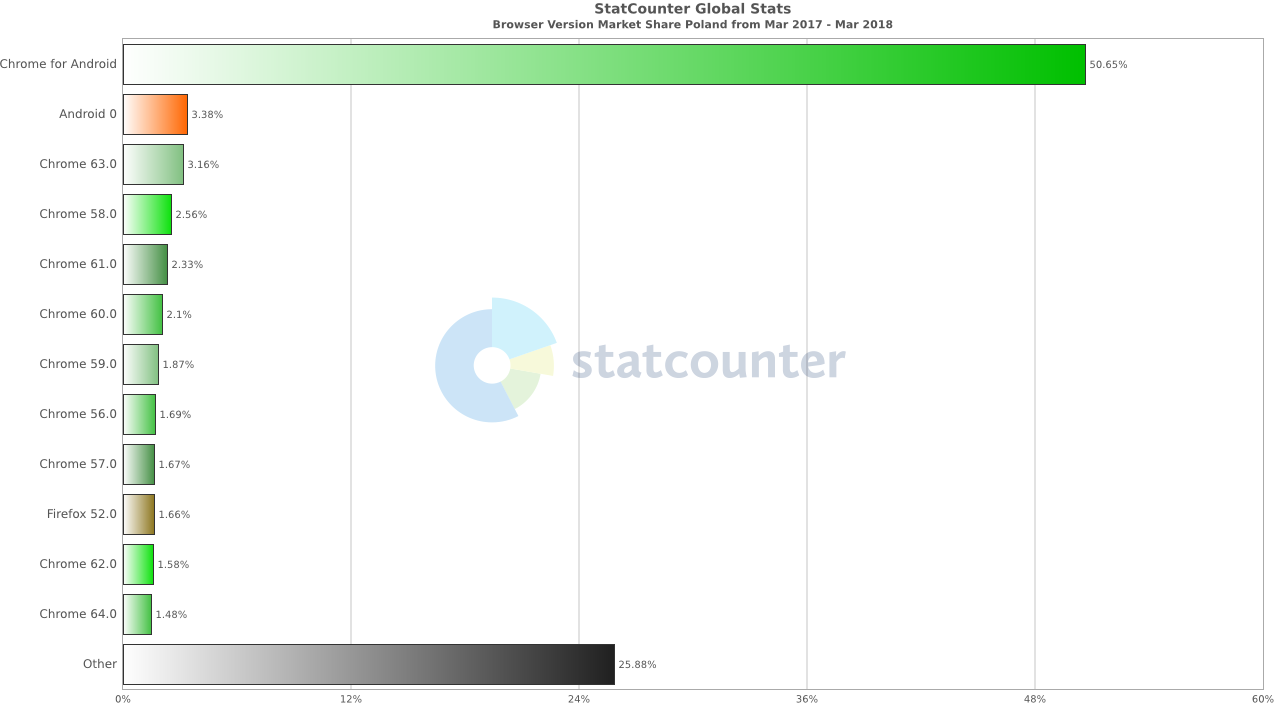
\includegraphics[scale=0.35]{chart}
\end{itemize}

\section{Schemat działania}

\subsection{Generowanie i wysyłanie danych}
Dane otrzymane przez użytkownika zostaną przekazane do napisanego przez nas API: send\_requests\_api. API wygeneruje zestaw wejść, które będą wysyłane do GA, a następnie za pomocą metody post z biblioteki requests wyśle je. 

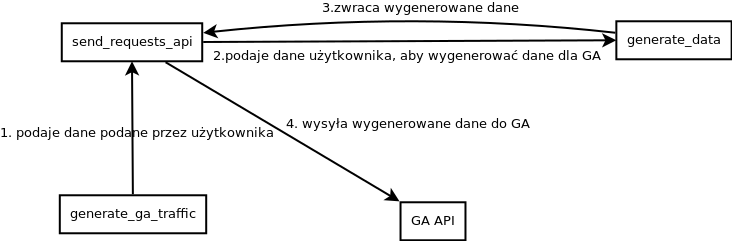
\includegraphics[scale=0.5]{connection_ga}

\subsection{Wykrywanie braku połączenia z internetem}
Jeśli send\_requests\_api przez 10 min. nie uda się wysłać żadnego requesta do GA API, w takim wypadku zostaje zatrzymane wysyłanie oraz zwrócony do generate\_ga\_traffic komunikat CONNECTION\_PROBLEM. Wtedy użytkownik zostaje o tym poinformowany i może wybrać jedną z trzech możliwości co chce robić dalej.

\end{document}
